\documentclass[letterpaper, 12pt, oneside]{tesis}

% Paquetes para idioma
\usepackage[spanish]{babel}
\usepackage[utf8]{inputenc}
\usepackage[fixlanguage]{babelbib}

% Otros paquetes instalados
% Básicos
\usepackage{natbib}
\usepackage{enumerate}

% Para dibujar figuras
\usepackage{tikz}

% Para cambiar el color de las letras
\usepackage{color}

% Para incluir código (básico)
\usepackage{verbatim}
\usepackage{fancyvrb}

% Para incluir hipervínculos
\usepackage{hyperref}
\hypersetup{urlcolor=blue, colorlinks=false}

% Para más símbolos matemáticos
\usepackage{amsmath}
\usepackage{amsthm}
\usepackage{amssymb}

% Para colocar teoremas en cajas
\usepackage{mdframed}

% Para texto Lorem Ipsum
\usepackage{blindtext}

% Para tener mas de un título
\usepackage{titling}

% Paquetes locales
% Puedes agregar paquetes locales (archivos .sty) en un subdirectorio % 'paquetes'.
% Utiliza la sintaxis \usepackage{paquetes/nombrePaquete}

% Todas las imágenes se cargan del subdirectorio 'img' por defecto.
\graphicspath{{img/}}

% Sangrías de 3 espacios (3 veces el espacio de la x)
\parindent 3ex

% Interlineado
\setlength{\baselineskip}{1.5pt}

% Interpárrafo
\setlength{\parskip}{16.5pt}

\topmargin 2cm

\renewcommand{\tablename}{Tabla}
\newcommand\listsymbolname{Lista de abreviaturas}

\begin{titlepage}
    \title{\vspace{-2cm} 
\includegraphics[width=1.2in]{./usb.png} \\[.2cm]
        \large Universidad Simón Bolívar \\
        Decanato de Estudios Profesionales \\
        Coordinación de Ingeniería de la Computación
        \vfill \LARGE \bfseries Desarrollo de nuevos componentes de las arquitecturas
        tecnológicas utilizadas por BBVA \vfill}
    \author{Por: \\
        Gustavo Antonio Gutiérrez Rondón \\[1.2cm]
        \bfseries{INFORME DE PASANTÍAS} \\
Presentado ante la Ilustre Universidad Simón Bolívar \\
como requisito parcial para optar al título de \\
Ingeniero de Computación}
    \date{\bfseries Sartenejas, Octubre de 2017}
\end{titlepage}

\begin{document}
\frontmatter
% Carátula
\maketitle

% Título
\begin{titlepage}
    \title{\vspace{-2cm} 
\includegraphics[width=1.2in]{./usb.png} \\[.2cm]
        \large Universidad Simón Bolívar \\
        Decanato de Estudios Profesionales \\
        Coordinación de Ingeniería de la Computación
        \vfill \LARGE \bfseries Desarrollo de nuevos componentes de las arquitecturas
        tecnológicas utilizadas por BBVA \vfill}
    \author{Por: \\
        Gustavo Antonio Gutiérrez Rondón \\[1.2cm]
        Realizado con la asesoría de: \\
        Prof. Federico Flaviani \\[1.2cm]
        \bfseries{INFORME DE PASANTÍAS} \\
Presentado ante la Ilustre Universidad Simón Bolívar \\
como requisito parcial para optar al título de \\
Ingeniero de Computación}
    \date{\bfseries Sartenejas, Octubre de 2017}
\end{titlepage}

\maketitle

\setstretch{1.3}

% Se incluye el acta de evaluación, verificar que se corresponda
% con el formato aceptado actualmente por el Decanato.
% Pagina del acta final
\begin{titlepage}
\begin{center}

% Upper part

\includegraphics[scale=0.5]{usb.png} \\

\textsc {\large UNIVERSIDAD SIMÓN BOLÍVAR} \\
\textsc{DECANATO DE ESTUDIOS PROFESIONALES\\
COORDINACIÓN DE INGENIERÍA DE LA COMPUTACIÓN}

\bigskip
\bigskip
\bigskip
\bigskip
\bigskip
\bigskip

% Title
\textsc{ACTA FINAL PROYECTO DE GRADO}

\bigskip
\bigskip

\textsc{\bfseries Desarrollo de nuevos componentes de las arquitecturas
        tecnológicas utilizadas por BBVA}
\bigskip
\bigskip
\bigskip
\bigskip

\begin{minipage}{\textwidth}
\centering
Presentado por: \\
\textsc{\bfseries Gustavo Antonio Gutiérrez Rondón} \\

\bigskip
\bigskip
\bigskip

Este Proyecto de Grado ha sido aprobado por el siguiente jurado examinador: \\

\bigskip
\bigskip

% Despues de cada line coloca el (los) nombre(s) de
% cada uno de los integrantes del jurado.
\line(1,0){200} \\
Federico Flaviani\\

\bigskip
\bigskip

\line(1,0){200} \\
@jurado1\\

\bigskip
\bigskip

\line(1,0){200} \\
@jurado2\\
\end{minipage}

\bigskip
\bigskip
\vfill

% Date/Fecha
{\large \bfseries Sartenejas, @día de @mes de 2017}

\end{center}
\end{titlepage}


% El resumen debe ser de una sola página
\addtotoc{Resumen}
\abstract{
\addtocontents{toc}{\vspace{1em}}

En este documento se detallan las actividades realizadas por el autor durante su
período de pasantías en el desarrollo de mejoras a las arquitecturas tecnológicas
utilizadas por el banco español BBVA.

BBVA en búsqueda de estandarizar y de facilitar el desarrollo de aplicaciones
define cuales son las plataformas a utilizar para implementar dichas aplicaciones.
Entre éstas plataformas se encuentran las arquitecturas ePhoenix, escrita en Java,
y la arquitectura Thin2, basada en el framework de Javascript Angular.

Fué responsabilidad del estudiante identificar posibles mejoras a éstas arquitecturas,
y luego diseñar e implementar dichas mejoras para ambas plataformas mencionadas.
Para la gestión del trabajo del estudiante se utilizó la metodología ágil de desarrollo
SCRUM.

El proyecto de pasantía dió como resultado final la certificación de conexiones
a bases de datos manejadas con PostgreSQL y MicrosoftSQLServer en la arquitectura
ePhoenix y el desarrollo de un componente reutilizable para crear tablas en la
arquitectura Thin2.

% Las palabras clave son generalmente los nombres de áreas de investigación a
% los cuales está asociado el trabajo. Generalmente son tres o cuatro.
\noindent \begin{small} \textbf{Palabras clave}: arquitectura, tecnológica, desarrollo, Java, Angular.
\end{small}

% Iniciar nueva página luego del resumen
\clearpage
\setstretch{1.3}

% Begin the Dedication page

\setstretch{1.3}  % Return the line spacing back to 1.3

\pagestyle{empty}  % Page style needs to be empty for this page

\dedicatory{
    \textbf{Dedicatoria} \bigskip

    A mi familia, quienes son la base sobre la que se levantan todos mis logros.
}

\addtocontents{toc}{\vspace{2em}}


% Agradecimientos
\acknowledgements{
\addtocontents{toc}{\vspace{1em}}
}
\clearpage

\pagestyle{fancy}

% Tabla de contenidos o índice
\lhead{\emph{Índice General}}
\tableofcontents

% Estos índices solamente se usan si el libro contiene figuras, tablas y
% algoritmos. Si alguno de estos no se utiliza, comentar o eliminar las líneas
% pertinentes.
\lhead{\emph{Índice de Figuras}}
\listoffigures

\lhead{\emph{Índice de Tablas}}
\renewcommand*\listtablename{Índice de Tablas}
\listoftables

%\lhead{\emph{Índice de Algoritmos}}
%\renewcommand*\listalgorithmname{Índice de algoritmos}
%\listofalgorithms

\setstretch{1.5}
\clearpage
\lhead{\emph{Lista de Abreviaturas}}
\listofsymbols{ll}
{

    % Aquí van las siglas
    \textbf{API} & \textbf{A}pplication \textbf{P}rogramming \textbf{I}nterface \\
    \textbf{JDBC} & \textbf{J}ava \textbf{D}ata\textbf{B}ase \textbf{C}onnectivity\\
    \textbf{JNDI} & \textbf{J}ava \textbf{N}aming and \textbf{D}irectory \textbf{I}nterface\\
    \textbf{SQL} & \textbf{S} \textbf{Q} \textbf{L} \\
    \textbf{HTML} & \textbf{H} \textbf{T} \textbf{M} \textbf{L} \\
    \textbf{OSGI} & \textbf{O}pen \textbf{S}ervice \textbf{G}ateway \textbf{I}nitiative\\
    &\\
    % \hline
    % &\\

    % % Aquí van los símbolos
    % $\iff$ & doble implicación, si y sólo si\\
    % $\Rightarrow$ & implicación lógica\\
    % $[u:=v]$ & sustitución textual de $u$ por $v$
}

%% ----------------------------------------------------------------
% End of the pre-able, contents and lists of things

\mainmatter
\pagestyle{fancy}

% Se incluye el cuerpo de la tesis en este documento.

\chapter*{Introducción}
\label{intro}
\lhead{\emph{Introducción}}
\addcontentsline{toc}{chapter}{Introducción}
% Organización del trabajo
% Se describe brevemente qué se hace en cada capítulo
El presente informe detalla el proceso llevado a cabo
para detectar, diseñar, implementar y probar mejoras a las arquitecturas
ePhoenix y Thin2 utilizadas en el banco español BBVA.

% Descripción del problema, de lo general hacia lo específico

El banco BBVA es una de las entidades líderes de España, con más de 10
millones de clientes y cerca de 30.000 empleados, prestando servicios
financieros a través de su red de 3200 oficinas (\cite{BBVA}). Dentro de
su área de tecnología cuenta con diferentes plataformas y arquitecturas
utilizadas con el objetivo de reducir el tiempo y homogeneizar el desarrollo.

Durante el proyecto se trabajó con dos de las arquitecturas mencionadas anteriormente.
La primera es la arquitectura ePhoenix que le permite a los equipos de desarrollo
realizar procesamientos por lotes y publicar servicios web. La segunda arquitectura
con la que se trabajó fue la arquitectura Thin2, la cual es un conjunto de librerías
basadas en Angular que le permite a los desarrolladores construir eficientemente
aplicaciones web.

\section*{Planteamiento del problema}

Con la finalidad de mantener las arquitecturas utilizadas en el banco lo
más actualizadas posibles es necesario un proceso constante de revisión y mejoras de
las mismas. Este proceso incluye una fase de levantamiento de requerimientos
para identificar fallas o posibles mejoras de las plataformas utilizadas. Luego,
una etapa de diseño de solución que solvente la deuda técnica detectada, para
finalmente pasar al desarrollo, prueba y despliegue de dicha solución.

Para contribuir con la actualización de ambas arquitecturas se debe realizar
una iteración de las etapas mencionadas sobre cada una de las plataformas para
así producir un evolutivo para ePhoenix y Thin2.

Durante el proceso de exploración se detectó que en la arquitectura ePhoenix sólo
se podían realizar conexiones a bases de datos de tipo Oracle, lo cual es una limitante
debido a que buena parte de la información manejada por el banco se encuentra en
bases de datos de otros manejadores, como PostgreSQL y Microsoft SQL Server.

Asimismo se detectó que en eld esarrollo de aplicaciones web existen operaciones
repetitivas y tediosas que enlentecen el proceso de desarrollo. Entre estas
operaciones se incluye la creación de tabla de datos, la cual involucra
un proceso bastante repetitivo.

\section*{Justificación e importancia}
Una de las constantes a la hora de desarrollar software es que los
requerimientos pueden cambiar a lo largo del tiempo. Ésto también
es cierto para los empleados encargados de desarrollar aplicaciones
dentro del banco BBVA. Debido a ésto es importante que las arquitecturas
que se utilicen para desarrollar soluciones tecnológicas, en específico
las arquitecturas ePhoenix y Thin2, se mantengan actualizadas y se mejoren
para poder satisfacer todas las necesidades de los desarrolladores.

La ventaja de mantener actualizadas las herramientas utilizadas es que le permite
a las empresas optimizar los procesos de desarrollo tecnológico que se realicen al
eliminar o mejorar los impedimentos que afectan al desarrollo de aplicaciones.

\section*{Objetivos}
A continuación se detallan el objetivo general y los objetivos específicos que
se buscan lograr en el desarrollo del proyecto.
% Objetivo general
\subsection*{Objetivo General}
El objetivo general de la pasantía es identificar posibles mejoras para las arquitecturas
de desarrollo ePhoenix y Thin2 utilizadas en el banco BBVA, y una vez
identificadas diseñar e implementar dichas mejoras para incorporarla dentro de los
estándares de arquitectura de la empresa y así enriquecer la experiencia de los
desarrolladores.
% Objetivos específicos
\subsection*{Objetivos Específicos}
\begin{itemize}
  \item Levantar información de uso de la arquitectura ePhoenix.
  \item Una vez identificada una carencia, diseñar una solución para
        mejorar la arquitectura.
  \item Implementar y probar la solución diseñada en ePhoenix.
  \item Levantar información de uso de la arquitectura Thin2.
  \item Una vez identificada una carencia, diseñar una solución para
        mejorar la arquitectura Thin2.
  \item Implementar y probar la solución diseñada en Thin2.
  \item Documentar y divulgar las mejoras implementadas para su
        posterior uso por los equipos de desarrollo del banco.
\end{itemize}

El documento se organiza en capítulos de la siguiente forma: la
Introducción al proyecto de Pasantías; en el Capítulo 1 se menciona
el contexto empresarial y el cargo ocupado en la
consultora Everis durante la pasantía; en el Capítulo 2 se explican
los fundamentos teóricos necesarios para la comprensión del problema y
la solución planteada; en el Capítulo 3 se detallan las tecnologías
implicadas en el proceso de desarrollo del proyecto; en el Capítulo 4 se
explica el funcionamiento de la metodología de gestión de proyectos utilizada
(SCRUM); en el Capítulo 5 se describen las actividades realizadas;
finalmente se le dan al lector las Conclusiones y recomendaciones.


% El número de capítulos varía. En mi libro fueron cuatro (sin contar
% introducción y conclusión).
\chapter{Entorno Empresarial}
\label{capitulo1}
\lhead{Capítulo 1. \emph{Entorno Empresarial}}

% De qué va a tratar el capítulo
% El capítulo 1 suele ser el marco teórico.

\section{@sección}
\begin{definition}
\label{definicion1}
, donde:
\begin{itemize}
\item $X$ es $\gamma - 2$.
\item $A$ es un conjunto de \textbf{cosas}.
\end{itemize}
\end{definition}

La Figura \ref{usb} muestra el símbolo de nuestra universidad.
\begin{figure}[h!]
\centering

\includegraphics[width=0.4\textwidth]{usb.png}
\caption[La popular \textit{cebolla}]{La popular \textit{cebolla}, símbolo de la USB.}
\label{usb}
\end{figure}

\begin{verbatim}
para escribir código
    básico
\end{verbatim}

\begin{Verbatim}[commandchars=\\\{\}, codes={\catcode`$=3\catcode`^=7}]
var x = 21;
if (esto_es_código) {
    imprimir(foo);
}
(lisp (listas (?paréntesis))
\end{Verbatim}

\begin{mdframed}
\begin{theorem}
\label{principal}
\textbf{Propiedades formales}
\end{theorem}
\end{mdframed}

\subsection{@subsección}
\subsubsection{@subsubsección}

La Figura \ref{grafo} lo muestra.

\shorthandoff{<>."}
\begin{figure}[h]
\begin{center}
\begin{tikzpicture}[shorten >=1pt, thick]%[shorten >=1pt,node distance=2cm,>=stealth',thick]
  \node [shape=circle,fill=black,inner sep=1.5pt,label=below:$s$] (q0) at (0,0) {};
  \node [shape=circle,fill=black,inner sep=1.5pt,label=below:$1$] (q1) at (2,0) {};
  \node [shape=circle,fill=black,inner sep=1.5pt,label=below:$t$] (q2) at (4,0) {};
  \path[->] (q0) edge (q1) (q1) edge (q2);
\end{tikzpicture}
\end{center}
\caption[@descripcionCorta]{@descripcionLarga}
\label{grafo}
\end{figure}

\begin{enumerate}[--]
\item 1
\item 2
\item 3
\end{enumerate}

\begin{tabular}{ll}
1 & 2\\ \hline
1 & 2\\
1 & 2\\
\end{tabular}

Tabla \ref{tabla:resultados}.

\begin{figure}[h]
\begin{alignat*}{1}
A\   & \longrightarrow B \mid C\\
\end{alignat*}
\caption[Gramática]{Gramática de un lenguaje.}
\label{gram}
\end{figure}

\begin{table}[h!]
\begin{center}
\begin{tabular}{llllll}
\multicolumn{4}{@{}c}{Nombre del experimento} \\
\midrule
              &    éxitos/intentos & tiempo (ms) & espacio (kB) \\
\midrule
instancia1          &        28/30 &    23 &       1.7 \\
instancia2          &        50/70 &    12 &       32.7 \\
\midrule
\end{tabular}
\end{center}
\caption[Resultados X/Y]{Resultados de X para Y}
\label{tabla:resultados}
\end{table}

\begin{equation}
\label{eq}
\Phi = (\forall x) (R x)
\end{equation}

En el Apéndice \ref{apendiceA} se encuentra.

\chapter{Marco Teórico}
\label{capitulo2}
\lhead{Capítulo 2. \emph{Marco Teórico}}

A continuación se detallan los aspectos teóricos sobre los cuales se basan
tanto las herramientas utilizadas en la pasantía como la solución propuesta
en este proyecto:

\section{API}
Un API (\emph{Application Programming Interface}) es un conjunto de comandos,
funciones, protocolos o métodos que le permiten a un programa comunicarse
con un sistema externo o librería. Las APIs permiten que varios sistemas
informáticos (Sistemas Operativos, aplicaciones, etc.) se comuniquen sin la
necesidad de exponer la funcionalidad interna de cada sistema. A su vez esto
le permite a los desarrolladores utilizar funcionalidades de otras aplicaciones
sin la necesidad de reescribir código (\cite{API}).

\section{Bases de datos relacional}

Una base de datos es un medio para almacenar y recuperar información. En términos simples
una base de datos relacional es aquella en la que la información es almacenada en tablas con
filas y columnas. Se le hace referencia a las tablas como relaciones ya que representa una
coleccion de objetos del mismo tipo. La habilidad de recuperar información relacionada de una
tabla es la base para el término Base de datos relacional (\cite{RELACIONAL}).

\section{Desarrollo Orientado a Componentes}

Este método de diseño de software establece que a la hora de construir un sistema
informático, las funcionalidades de éste sean separadas en unidades más pequeñas
llamadas componentes. Un componente es una pieza de software que ofrece a través
de una interfaz un servicio predefinido y que es capaz de comunicarse con otros
componentes (\cite{COMPONENT}). Esta estrategia de desarrollo trae como resultado
software que puede ser reutilizado con mayor facilidad y que es fácilmente escalable
agregando futuros componentes que agreguen nuevas funcionalidades. Además, facilita la
mantenibilidad del código, debido a que la encapsulación de las funcionalidades permite
detectar con mayor facilidad de donde proviene una falla.

\section{Modelo Vista Controlador}
Modelo-Vista-Controlador (MVC) es un patrón de diseño de software, especialmente útil
para diseñar interfaces de usuario. Se basa en la separación de los datos y lógica de
negocio, la interfaz gráfica a mostrar y el módulo encargado de atender y responder a
los eventos generados por el usuario en tres componentes distintos (\cite{MVC}). Estos
componentes quedan definidos de la siguiente manera:

\begin{itemize}
  \item \textbf{Modelo}: se encarga de representar los datos que maneja el sistema y
  la funcionalidad asociada que tengan estos modelos.
  \item \textbf{Vista}: está a cargo de mostrar la representación visual del modelo
  para que el usuario interactúe fácilmente con el sistema.
  \item \textbf{Controlador}: es el módulo encargado de coordinar las vistas con el modelo.
  Para ello atiende los eventos que pueda generar el usuario para luego actualizar
  adecuadamente la vista y el modelo.
\end{itemize}

Este patrón de arquitectura de software se ha vuelto bastante común en el desarrollo
de interfaces de usuario por su ventajas en cuanto a reutilización y mantenibilidad
del código.

\chapter{Marco Tecnológico}
\label{capitulo3}
\lhead{Capítulo 3. \emph{Marco Tecnológico}}

En este capítulo se mencionan las herramientas utilizadas para el desarrollo
del proyecto de pasantía. Dichas herramientas son descritas brevemente y se menciona
su uso dentro de la solución planteada.

\section{Java}

Java es un lenguaje de programación de propósito general, concurrente, basado en clases
y orientado a objetos. Está diseñado para ser lo suficientemente sencillo para
que muchos programadores puedan alcanzar fluidez en el lenguaje. (\cite{JAVA})

\section{OSGI}

OSGI (\emph{(Open Service Gateway Initiative)}) es un conjunto de especificaciones
que definen un sistema dinámico formado por componentes
para Java. Estas especificaciones permiten un modelo de desarrollo donde las aplicaciones
son dinámicamente compuestas por muchos componentes reutilizables (\cite{OSGI}).

En la figura \ref{layers} se describe el modelo por capas definido por OSGI:

\begin{figure}[h!]
\centering
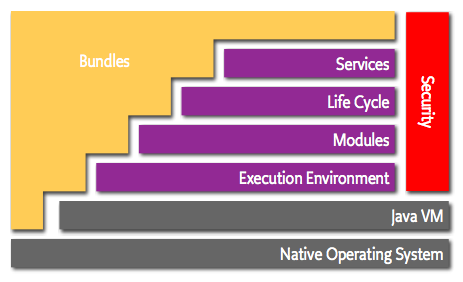
\includegraphics[width=0.4\textwidth]{layering-osgi}
\caption[Capas de OSGI]{Modelo por capas definido en OSGI. (\cite{OSGI})}
\label{layers}
\end{figure}

La siguiente lista contiene una breve descripción de los términos:
\begin{itemize}
\item \textbf{Bundles}: los Bundles son los componentes de OSGI hechos por los desarrolladores.
\item \textbf{Servicios}: la capa de servicios conecta bundles de una manera dinámica intercambiando objectos Java.
\item \textbf{Ciclo de vida}: el API para instalar, arrancar, detener, actualizar y desinstalar un bundle.
\item \textbf{Módulos}: la capa que define como un bundle puede importar y exportar código.
\item \textbf{Seguridad}: la capa que determina los aspectos de seguridad.
\item \textbf{Ambiente de Ejecución}: define que métodos y clases están disponibles en una plataforma específica.
\end{itemize}


\section{Apache Felix}

Apache Felix es un esfuerzo de la comunidad Apache para implementar la especificación de
la plataforma OSGI bajo la licencia Apache. La especificación OSGI es ideal para
cualquier proyecto interesado en los principios de modularidad, desarrollo orientado
a componentes y desarrollo orientado a servicios (\cite{FELIX}).

\section{JDBC}

El \emph{API} JDBC (\emph{Java Database Connectivity}) es el estándar en la industria
para conectividad independiente del manejador de base de datos entre programas escritos en
Java y una gran variedad de bases de datos (\cite{JDBC}). Para cada uno de los manejadores
de base de datos que se desean conectar a través de un programa Java deberá existir una implementación
del estándar JDBC, también llamado Driver, que le permite al programa comunicarse a través del
API con el manejador de base de datos.

\section{Base de datos Oracle}

La base de datos Oracle es un sistema de manejo de base de datos relacional (\cite{ORACLE})
producido y mantenido por Oracle Corporation.

\section{PostgreSQL}

PostgreSQL es un poderoso sistema de bases de datos relacional. Tiene más de
15 años de desarrollo activo y una arquitectura que se ha ganado la reputación de tener
integridad de datos, confiabilidad y correctitud de datos (\cite{POSTGRE}).

\section{Microsoft SQL Server}
Microsoft SQL Server es un sistema de manejo de bases de datos relacional desarrollado por
Microsoft.

\section{Arquitectura ePhoenix}

Construido sobre la base de Apache Felix, la arquitectura ePhoenix le brinda a los
equipos de desarrollo del BBVA todas las herramientas necesarias para desarrollar programas
que realicen procesamiento por lotes o publiquen servicios web. Cuando un equipo de
desarrolladores se disponga a realizar aplicaciones con esta arquitectura se le despliegan
en un servidor dedicado Apache Félix junto con los bundles que conforman ePhoenix para
que los desarrolladores desplieguen sus propios bundles que implementen su lógica de negocio.

Abarcar todas las funcionalidades que ofrece la arquitectura escapa del alcance del
proyecto de pasantías, por lo que se trabajará con los componentes de ePhoenix
que se encargan de realizar las conexiones a bases de datos usando JDBC.

\section{HTML}

HTML, que significa Lenguaje de Marcado para Hipertextos (HyperText Markup Language)
es el elemento de construcción más básico de una página web y se usa para crear y
representar visualmente una página web. Determina el contenido de la página web,
pero no su funcionalidad (\cite{HTML}).

\section{Javascript}

JavaScript es un lenguaje ligero e interpretado, orientado a objetos, más conocido
como el lenguaje de script para páginas web. Es un lenguaje script multi-paradigma, dinámico,
soporta estilos de programación funcional, orientada a objetos e imperativa (\cite{JS}).

\section{Node.js}
Node.js es un entorno de ejecución para JavaScript construido con el motor de JavaScript V8
de Chrome. Node.js usa un modelo de operaciones de entrada y salida sin bloqueo y orientado a eventos.
El ecosistema de paquetes de Node.js, npm, es el ecosistema mas grande de librerías
de código abierto en el mundo (\cite{NODE}).

\section{JSON}
JSON (\emph{JavaScript Object Notation}) es un formato de intercambio de datos ligero.
Esta diseñado para ser fácil de leer y escribir por humanos y fácil de parsear y generar
por las máquinas (\cite{JSON}).

\section{Angular}
Angular es una plataforma escrita en JavaScript que facilita el proceso
de crear aplicaciones para la web. Angular combina plantillas declarativas, inyección de dependencias
y buenas prácticas integradas para solucionar problemas a la hora de desarrollar (\cite{ANGULAR}).
Además, al presentar una arquitectura que combina el desarrollo orientado a componentes
y el patrón de diseño MVC, Angular ofrece grandes ventajas en cuanto a mantenibilidad
y reusabilidad de código.

\section{Arquitectura Thin2}

A diferencia de ePhoenix, Thin2 no está basado en OSGI.
Para Thin2 se tomó como base el framework de aplicaciones web Angular. Partiendo
de la capacidad de Angular de definir componentes reutilizables se le ofrecen a los
equipos de desarrollo varios elementos predefinidos para realizar las tareas más
comunes a la hora de escribir una página web. Entre estos componentes se pueden
mencionar el componente para obtener configuraciones de un servidor o el que implementa
la autenticación y autorización propia manejada dentro de BBVA.

En la práctica, la arquitectura Thin2 está conformada por un conjunto de librerías
escritas con Angular puestas a la disposición de los equipos de desarrollo a través
del repositorio interno de BBVA. Una vez descargadas estas librerías junto con
Angular, los desarrolladores pueden utilizar los componentes predefinidos en la
arquitectura para realizar sus aplicaciones web.

\section{Herramientas para la gestión del proyecto}

Aparte de las tecnologías utilizadas para desarrollar el proyecto se utilizaron
las siguientes herramientas para la gestión de la pasantía y el control de versiones:

\subsection{Dimensions CM}

Dimensions CM is un gestor de cambios y configuraciones que disminuye eficientemente
la complejidad del desarrollo paralelo, integrando y automatizando prácticas de desarrollo
(\cite{DIMENSIONS}).

Dimensions CM es la herramienta utilizada en el BBVA para el control de versiones, control de
calidad y el despliegue de aplicaciones.

\subsection{Jira}

Jira Software es una herramienta de gestión de proyectos para equipos ágiles (\cite{JIRA}).
Entre sus características ofrece una manera sencilla de manejar y visualizar
las tareas asignadas mediante la metodología de trabajo SCRUM.

\chapter{@nombreCapítulo}
\label{capitulo4}
\lhead{Capítulo 4. \emph{@nombreCapítulo}}

\Blindtext

\chapter{Desarrollo del Proyecto}
\label{capitulo4}
\lhead{Capítulo 4. \emph{Desarrollo del Proyecto}}

En este capítulo se detallan las actividades realizadas para el
desarrollo del proyecto de pasantías. El proyecto fue realizado
mediante la metodología de desarrollo SCRUM descrita en el capítulo
anterior, con \emph{Sprints} de dos semanas de duración, por lo
que la pasantía quedó dividida en 10 \emph{sprints}. El proyecto
se divide en dos grandes fases: el desarrollo del evolutivo para ePhoenix
y el desarrollo del evolutivo para Thin2. A su vez, cada etapa contempla
las fases de levantamiento de información, análisis, diseño, implementación,
pruebas y despliegue de los artefactos desarrollados. A continuación se
expone por \emph{Sprint} los objetivos y las actividades realizadas.

\section{Primer Sprint}

\subsection{Objetivos}
\begin{itemize}
\item Estudio de las herramientas utilizadas en el banco.
\end{itemize}
\subsection{Actividades}
\subsubsection{Leer documentación de las arquitecturas}
Para ambas arquitecturas (ePhoenix y Thin2) existe documentación interna del BBVA
para su uso, la cual fué leída por el estudiante.
\subsubsection{Asistir a formaciones sobre el uso de las arquitecturas}
Dentro del banco se ofrecen formaciones a los nuevos equipos de desarrollo
sobre como utilizar las arquitecturas del banco para desarrollar aplicaciones con
ellas. El pasante asisitió a una formación para cada arquitectura para tener
una perspectiva más práctica sobre el uso de las plataformas.
\subsubsection{Realizar tutoriales}
Para asentar los conocimientos adquiridos en las actividades previas se propuso
realizar tutoriales sobre las herramientas a utilizar. Para Thin2 se realizó un
tutorial de Angular (el \emph{framework} sobre el cual se basa Thin2) y para ePhoenix
se siguieron las guías mencionadas en la documentación para realizar un bundle sencillo
de procesamiento por lotes.

\section{Segundo Sprint}

\subsection{Objetivos}
\begin{itemize}
  \item Levantar información sobre necesidades en ePhoenix.
  \item Detectar una mejora o carencia en la arquitectura.
  \item Diseñar una solución para dicha carencia.
\end{itemize}
\subsection{Actividades}
\subsubsection{Reunión con distintos equipos de desarrollo}
Se concretaron reuniones breves con los distintos equipos de desarrollo del banco
para que pudieran plantear que características piensan que se podrían mejorar o agregar a la
arquitectura ePhoenix.
\subsubsection{Análisis de la información recolectada}
Tomando en cuenta los comentarios recibidos en las reuniones informativas se llegó
a la conclusión que existía la necesidad de poderse conectar a bases de datos de otros
manejadores distintos a Oracle.
\subsubsection{Diseño de solución para conectar con otros manejadores de Base de datos}
Una vez analizados los \emph{bundles} que toman parte en la realización de conexiones a bases
de datos se determinó que se necesita crear un bundle para cada driver de conexión a base de
datos. Después de creados estos componentes, se debe implementar un \emph{bundle} que permita
la inclusión de estos drivers en el componente de conexión a base de datos. Finalmente se deberá
modificar la interfaz de administración de ePhoenix para permitirle a los usuarios
crear conexiones de distintos proveedores de base de datos.

\section{Tercer Sprint}

\subsection{Objetivos}
\begin{itemize}
  \item Implementar los \emph{bundles} necesarios para realizar conexiones.
\end{itemize}
\subsection{Actividades}
\subsubsection{Convertir los drivers de PostgreSQL y Microsoft SQL en \emph{bundles}}
Para esto se descargaron los drivers de PostgreSQL y Microsoft SQL disponibles en
internet y se realizaron las modificaciones necesarias para que sea reconocido por
OSGI como un bundle.
\subsubsection{Implementar los \emph{bundles} de tipo fragmento}
Luego, el pasante pasó a crear los \emph{bundles} responsables de comunicar los
drivers de los manejadores de base de datos con el componente que crea las conexiones
a base de datos.
\subsubsection{Probar las conexiones creadas}
Una vez creados los artefactos mencionados en las actividades pasadas se procedió
a crear un \emph{bundle} de prueba que realizara una conexión con una base de datos
PostgreSQL y una manejada con Microsoft SQL Server y reportara éxito en caso de
realizar la conexión satisfactoriamente.

\section{Cuarto Sprint}

\subsection{Objetivos}
\begin{itemize}
  \item Modificar los bundles de la interfaz de administración para crear nuevas
  conexiones.
\end{itemize}
\subsection{Actividades}
\subsubsection{Agregar un campo desplegable que permita elegir el tipo de base de datos}
Los equipos de desarrollo cuentan con una interfaz administrativa para la creación y configuración
de conexiones para sus aplicaciones. En las figuras del apéndice \ref{apendiceA} se pueden ver las
modificaciones realizadas a la interfaz.
\subsubsection{Modificar el bundle que crea la configuracion para la conexión}
Adicionalmente existe otro \emph{bundle} que es el encargado de una vez configurada la conexión
en el tablero administrativo, cree los archivos de configuración necesarios para establecer
la conexión a la base de datos.

\section{Quinto Sprint}

\subsection{Objetivos}
\begin{itemize}
  \item Realizar pruebas sobre los bundles
  \item Desplegar los bundles implementados para su utilización.
\end{itemize}
\subsection{Actividades}
\subsubsection{Realización de pruebas}
Para garantizar el correcto funcionamiento de los bundles desarrollados
se probó que se realizaran correctamente las conexiones a base de datos en distintos
entornos y con distintas bases de datos.
\subsubsection{Desplegar con Dimensions los bundles}
Una vez implementados y probados los componentes necesarios, se procedió a publicar
el desarrollo a través de la herramienta \emph{Dimensions} para que esté disponible
en los servidores de producción para su uso por los equipos de desarrollo.
\subsubsection{Documentar la solución planteada}
Se actualizó la documentación interna de la arquitectura ePhoenix para que reflejara
la posibilidad de crear conexiones de bases de datos de otros proveedores con pasos
detallados de como realizar estas conexiones.

\section{Sexto Sprint}

\subsection{Objetivos}
\begin{itemize}
  \item Levantar información sobre necesidades en Thin2.
  \item Detectar una mejora o carencia en la arquitectura.
  \item Diseñar una solución para dicha carencia.
\end{itemize}
\subsection{Actividades}
\subsubsection{Reunión con distintos equipos de desarrollo}
Al igual que con ePhoenix se llevaron acabo reuniones con los desarrolladores
de aplicaciones web para que pudieran dar recomendaciones sobre que funcionalidad
mejoraría su experiencia a la hora de crear aplicaciones.
\subsubsection{Análisis de la información recolectada}
Después de recolectada y analizada la información se hizo notar que una operación
bastante común a la hora de realizar aplicaciones web para el banco era mostrar
información en tablas. Este proceso a su vez suele ser tedioso y con resultados
bastante heterogéneos. Es por esto que se decidió crear un componente para Thin2
que facilitara la creación de tablas de datos.
\subsubsection{Diseño de solución para facilitar la creación de tablas de datos}
Para facilitar la creación de tablas se decidió crear un componente reutilizable
de Angular. Este componente, llamado \emph{th2-grid-component}, recibiría como
parámetros de entrada un objeto JSON que describe las columnas a crear, un objeto
JSON con la información a mostrar en la tabla, y una función opcional que determina
el comportamiento a realizar si se hace click en una celda de la tabla.

\section{Séptimo Sprint}

\subsection{Objetivos}
\begin{itemize}
  \item Implementar versión básica del componente de tablas.
\end{itemize}
\subsection{Actividades}
\subsubsection{Implementar primera versión del componente}
En esta primera iteración se le dió mayor prioridad a desarrollar las características
básicas del componente, que son poder crear tablas con un formato sencillo y que muestren
la información deseada.


\section{Octavo Sprint}

\subsection{Objetivos}
\begin{itemize}
  \item Implementar segunda fase del componente.
\end{itemize}
\subsection{Actividades}
\subsubsection{Implementar mejora que permita darle formato a las tablas.}
Se mejoró el componente para que pudiera recibir clases HTML para cada columna
para que el desarrollador pueda darle formatos específicos a las columnas y a las celdas
de la tabla.
\subsubsection{Permitir que el componente reciba por parámetro la función a ejecutar.}
Luego se pasó a implementar la útlima funcionalidad deseada, que permite que el
componente reciba la función a ejecutar si se hace click sobre una celda de la tabla.

\section{Noveno Sprint}

\subsection{Objetivos}
\begin{itemize}
  \item Desplegar el componente en el repositorio de artefactos del banco.
  \item Documentar y divulgar la creación del nuevo componente para Thin2.
\end{itemize}
\subsection{Actividades}
\subsubsection{Desplegar el componente desarrollado a través de Dimensions}
El componente implementado fue desplegado a través de Dimensions para que esté
disponible en el repositorio de artefactos interno del banco.
\subsubsection{Actualizar documentación sobre la arquitectura}
Se llevó acabo la actualización de la documentación interna del banco sobre
Thin2 para agregar un inciso sobre el nuevo componente implementado con
una breves instrucciones sobre como utilizar dicha funcionalidad.

\section{Décimo Sprint}

\subsection{Objetivos}
\begin{itemize}
  \item Crear una aplicación de ejemplo que muestre el uso del componente de tablas.
\end{itemize}
\subsection{Actividades}
\subsubsection{Desarrollar una pequeña aplicación web de ejemplo}
Para facilitar el uso del componente de tablas por parte de los equipos de
desarrollo el pasante implementó una pequeña aplicación web que ejemplificara
como utilizar el componente desarrollado. En el apéndice \ref{apendiceB} se muestra parte
del código utilizado para crear una tabla y el resultado correspondiente en el navegador.


\chapter{Conclusiones y Recomendaciones}
\label{conclusiones}
\lhead{\emph{Conclusiones y Recomendaciones}}

% Incluir recomendaciones para trabajos futuros


% El estilo de la bibliografía es AAAI, definido en el archivo aaai.bst.
\label{Bibliography}
\bibliography{bibliografia}
\lhead{\emph{Bibliografía}}
\bibliographystyle{aaai}
\addtocontents{toc}{\vspace{2em}}

% Apéndices
\appendix
\chapter{Cambios en la interfaz administrativa de ePhoenix}
\label{apendiceA}
\lhead{Apéndice A. \emph{Cambios en la interfaz administrativa de ePhoenix}}

% En los apéndices se incluye cualquier información que no sea esencial para la
% comprensión básica del trabajo, pero provea ejemplos y casos de estudio
% extendidos que permitan un análisis más exhaustivo.

\begin{figure}[h!]
\centering
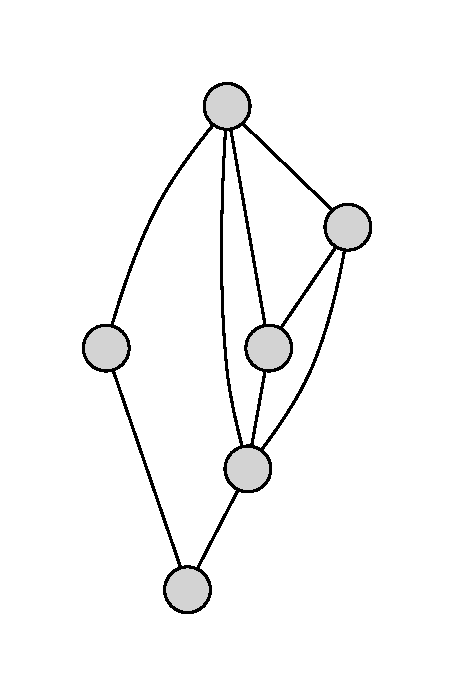
\includegraphics[width=0.5\textwidth]{grafo}
\caption[Grafo]{Grafo gris.}
\label{imagen:grafo}
\end{figure}

\begin{figure}[h!]
\centering
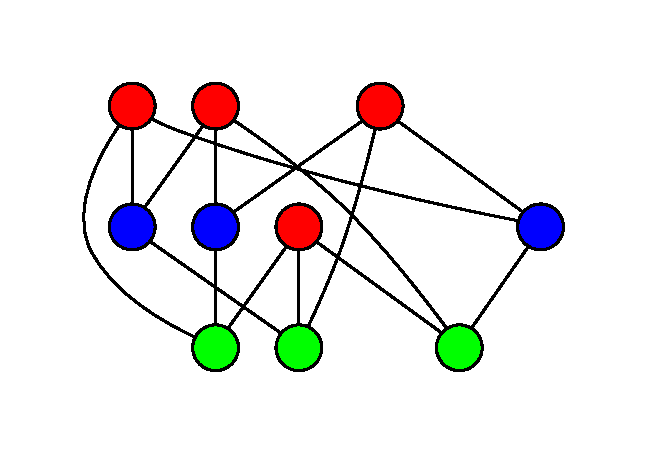
\includegraphics[width=\textwidth]{grafocolor}
\caption[Grafo coloreado (esto sale en la tabla de contenidos)]{Grafo con color.}
\label{imagen:grafodecolores}
\end{figure}

\chapter{Pantallazos de la aplicación de ejemplo para Thin2}
\label{apendiceB}
\lhead{Apéndice B. \emph{Pantallazos de la aplicación de ejemplo para Thin2}}

\begin{figure}[h!]
\centering
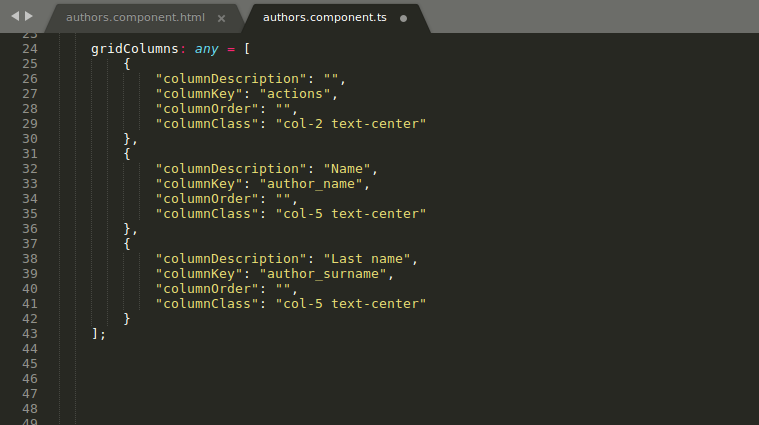
\includegraphics[width=\textwidth]{author-config}
\caption[Configuración de tabla sencilla]{Configuración de una tabla sin función.}
\label{author:1}
\end{figure}

\begin{figure}[h!]
\centering
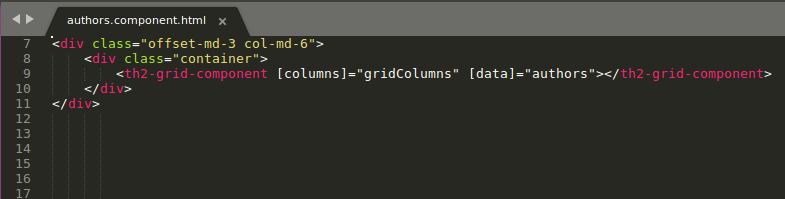
\includegraphics[width=\textwidth]{author-html}
\caption[Código html de tabla sencilla]{Código html utilizado para crear una tabla sin función.}
\label{author:2}
\end{figure}

\begin{figure}[h!]
\centering
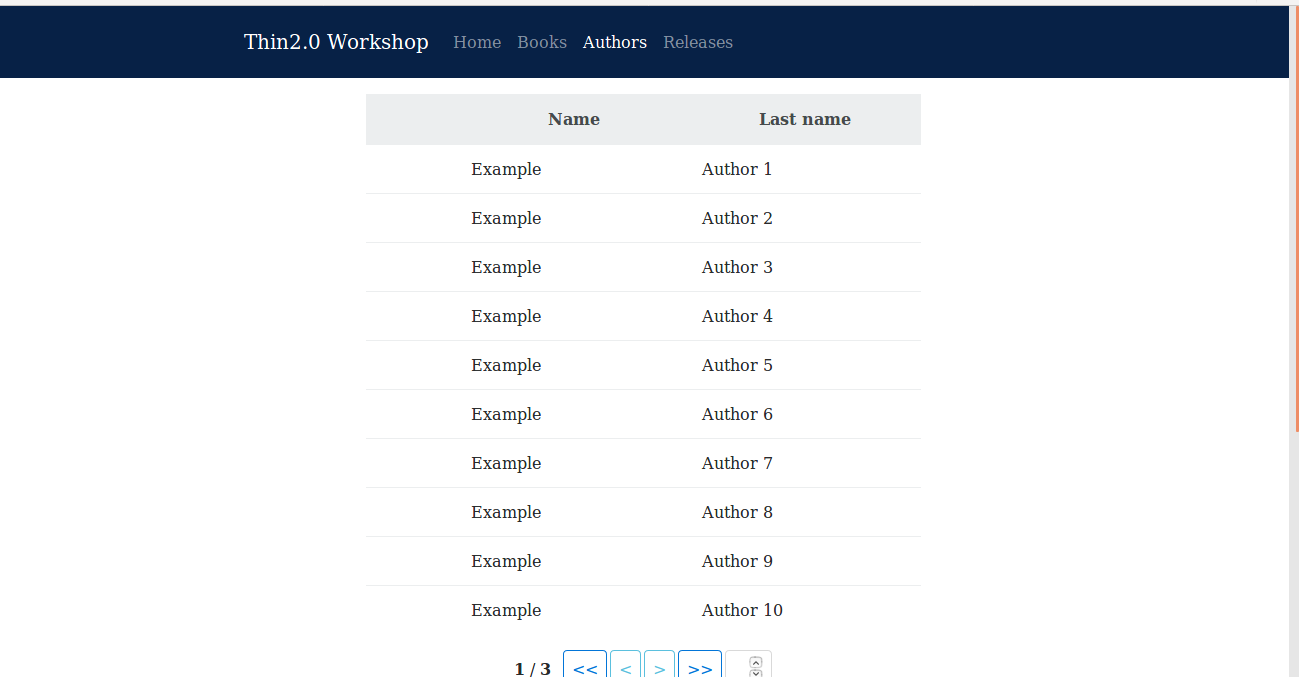
\includegraphics[width=\textwidth]{author-resultados}
\caption[Tabla sencilla en aplicación]{Resultado de la tabla realizada en la aplicación.}
\label{author:3}
\end{figure}

\begin{figure}[h!]
\centering
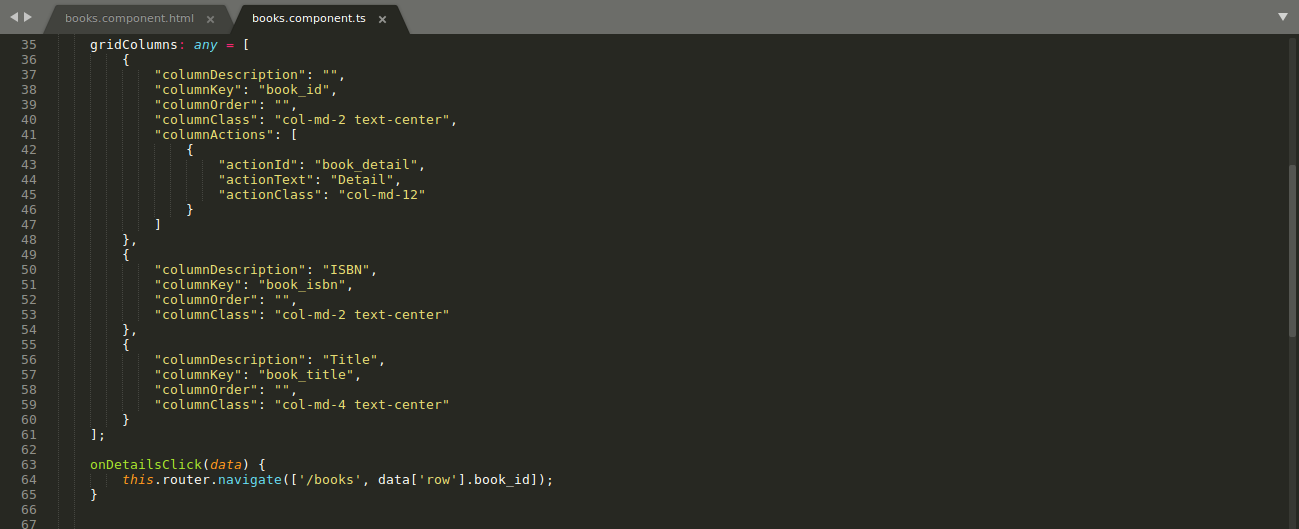
\includegraphics[width=\textwidth]{books-config}
\caption[Configuración de tabla con evento]{Configuración de una tabla con una función asociada.}
\label{books:1}
\end{figure}

\begin{figure}[h!]
\centering
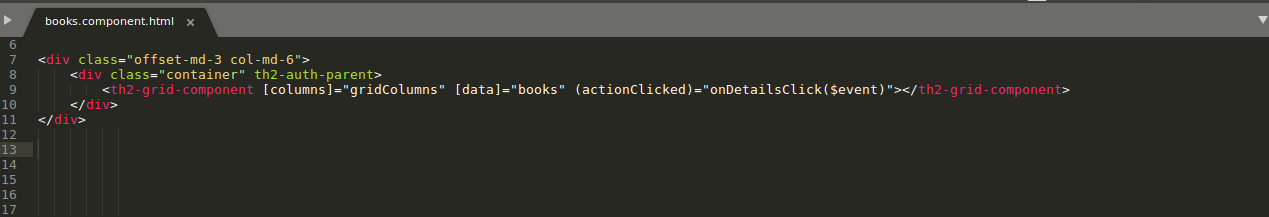
\includegraphics[width=\textwidth]{books-html}
\caption[Código html de tabla con evento]{Código html utilizado para crear una tabla con una función asociada.}
\label{books:2}
\end{figure}

\begin{figure}[h!]
\centering
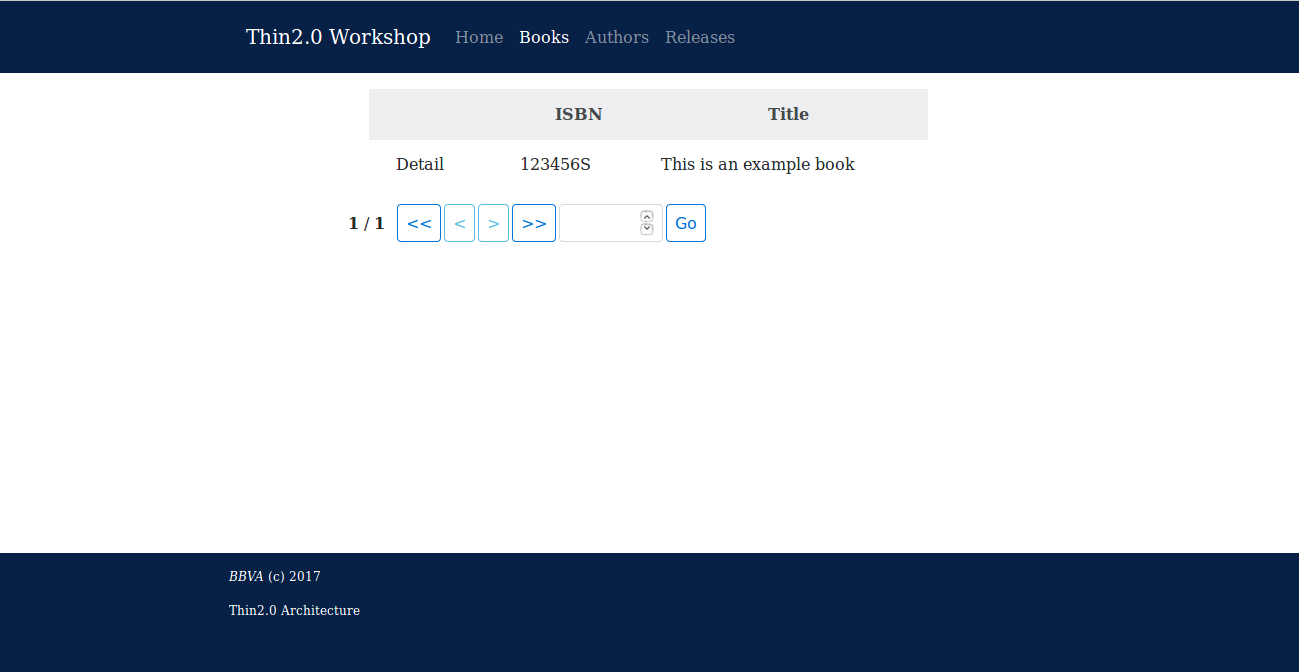
\includegraphics[width=\textwidth]{books-result}
\caption[Tabla con evento en aplicación]{Tabla con función asociada resultante en la aplicación.}
\label{books:3}
\end{figure}

\begin{figure}[h!]
\centering
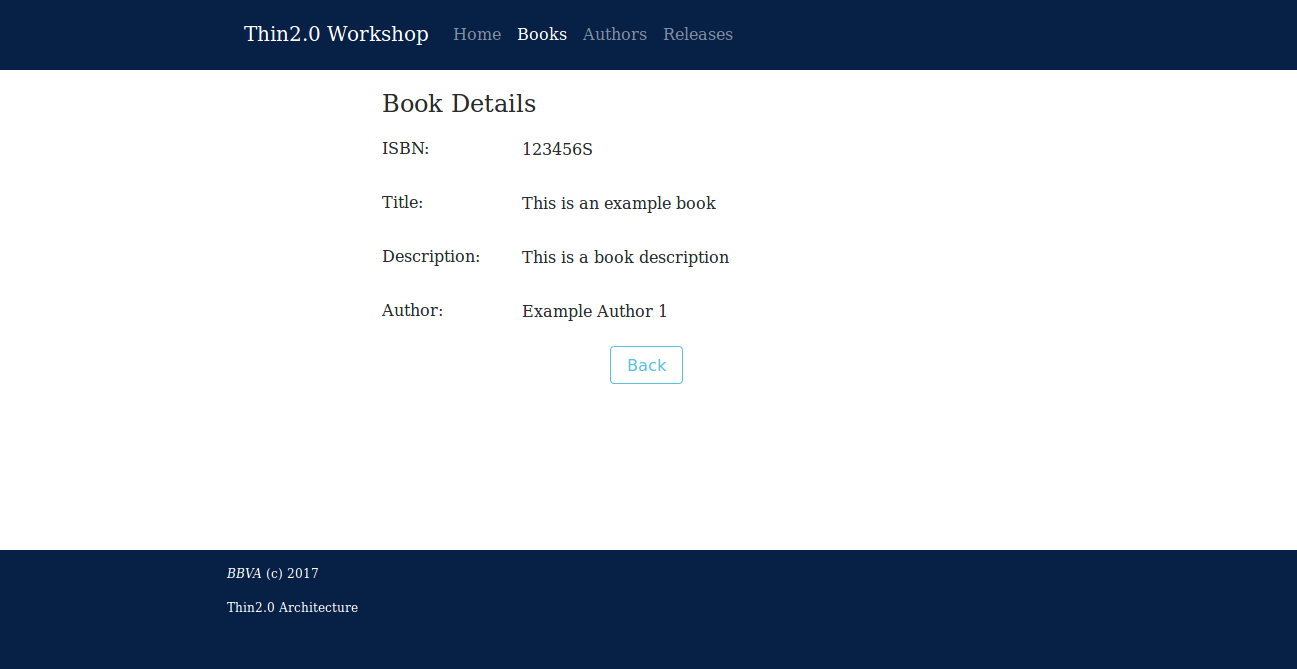
\includegraphics[width=\textwidth]{book-detail}
\caption[Página al hacer click en la tabla]{Cambio en la aplicación al ejecutar la función asociada a la celda.}
\label{books:4}
\end{figure}

\addtocontents{toc}{\vspace{2em}}

\backmatter

\end{document}
